\begin{pastexam}[label={px:ntust-114-ice-14}]{臺科大資工所 114 學年度 第 14 題}
（填空；每格 5 分）

(15\%) Given a weighted undirected graph, use Prim's algorithm starting from vertex B to find a
minimum spanning tree (MST). What is the total weight of this MST? \blank{E} Then, from vertex E,
perform a Depth First Search (DFS) and write down the order in which the vertices are visited.
\blank{F} Next, from the same vertex E, conduct a Breadth First Search (BFS) and record that
visitation order. \blank{G} In both the DFS and BFS traversals, if multiple edges are available at
any point, choose the one with the lowest weight first.

\begin{center}
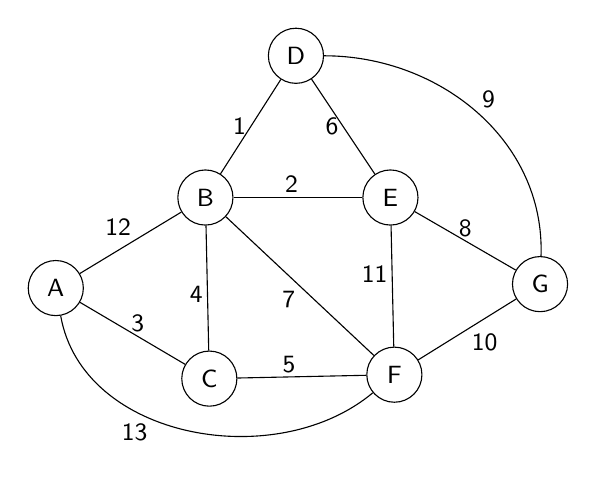
\begin{tikzpicture}[v/.style={circle,draw,minimum size=7mm,inner sep=0pt,font=\small\sffamily},
  w/.style={font=\small\sffamily,inner sep=1.5pt}]
\node[v] (A) at (0,0) {A};
\node[v] (B) at (1.9,1.15) {B};
\node[v] (C) at (1.95,-1.15) {C};
\node[v] (D) at (3.05,2.95) {D};
\node[v] (E) at (4.25,1.15) {E};
\node[v] (F) at (4.3,-1.1) {F};
\node[v] (G) at (6.15,0.05) {G};
\draw (B)--node[w,left]{1}(D);
\draw (D)--node[w,left]{6}(E);
\draw (B)--node[w,above,pos=0.45]{2}(E);
\draw (A)--node[w,above left,pos=0.55]{12}(B);
\draw (A)--node[w,above,pos=0.55]{3}(C);
\draw (B)--node[w,left,pos=0.55]{4}(C);
\draw (B)--node[w,below left,pos=0.5]{7}(F);
\draw (E)--node[w,left,pos=0.4]{11}(F);
\draw (E)--node[w,above,pos=0.5]{8}(G);
\draw (C)--node[w,above,pos=0.4]{5}(F);
\draw (F)--node[w,below right,pos=0.5]{10}(G);
\draw (D) to[out=0,in=88] node[w,above right,pos=0.5]{9} (G);
\draw (A) to[out=-80,in=-140] node[w,below left,pos=0.4]{13} (F);
\end{tikzpicture}
\end{center}
\end{pastexam}

\begin{pastsoln}
答案：(E) $23$；(F) E, B, D, G, F, C, A；(G) E, B, D, G, F, C, A。

(E) 屬於資結書第~24~章（最小生成樹），(F)(G) 屬於第~21~章；(F)(G) 佔 $10$ 分，所以整題放在本章。

圖的邊（權重）：B--D 1，B--E 2，A--C 3，B--C 4，C--F 5，D--E 6，B--F 7，E--G 8，D--G 9，F--G 10，
E--F 11，A--B 12，A--F 13。

\textbf{(E) Prim，從 B 開始}（資結書第~24.3~節）：每一步在「一端在樹裡、一端不在」的邊裡選最輕的。
\begin{center}
\small
\begin{tabular}{clll}
\toprule
步 & 樹裡的點 & 當時較輕的幾條跨越邊 & 選 \\
\midrule
1 & B & B--D 1, B--E 2, B--C 4, B--F 7 & B--D 1 \\
2 & B, D & B--E 2, B--C 4, D--E 6, B--F 7 & B--E 2 \\
3 & B, D, E & B--C 4, B--F 7, E--G 8, D--G 9 & B--C 4 \\
4 & B, C, D, E & A--C 3, C--F 5, B--F 7, E--G 8 & A--C 3 \\
5 & A, B, C, D, E & C--F 5, B--F 7, E--G 8, D--G 9 & C--F 5 \\
6 & A, B, C, D, E, F & E--G 8, D--G 9, F--G 10 & E--G 8 \\
\bottomrule
\end{tabular}
\end{center}
總權重 $1 + 2 + 4 + 3 + 5 + 8 = 23$。 （權重各不相同，最小生成樹唯一，Kruskal 也會得到同樣六條邊。）

\textbf{(F) DFS，從 E 開始}（資結書第~21.4~節）：每到一個點，依權重由小到大看它的鄰點，遇到還沒拜訪的就
立刻走進去；都拜訪過了就退回上一個點。
\begin{itemize}
\item E 的鄰點依權重：B 2、D 6、G 8、F 11。 走到 B。
\item B：D 1、E 2（已拜訪）、C 4、F 7、A 12。 走到 D。
\item D：B 1、E 6 都已拜訪，G 9。 走到 G。
\item G：E 8、D 9 已拜訪，F 10。 走到 F。
\item F：C 5。 走到 C。
\item C：A 3。 走到 A。
\item A 的鄰點 C、B、F 都已拜訪，一路退回 E，結束。
\end{itemize}
拜訪順序：E, B, D, G, F, C, A。

\textbf{(G) BFS，從 E 開始}（資結書第~21.3~節）：取出佇列前端的點，把它還沒拜訪過的鄰點依權重由小到大
標記並放進佇列。
\begin{center}
\begin{tabular}{lll}
\toprule
取出 & 新加入（依權重） & 佇列 \\
\midrule
（開始） & E & E \\
E & B 2, D 6, G 8, F 11 & B, D, G, F \\
B & C 4, A 12（D、E、F 已在） & D, G, F, C, A \\
D, G, F, C, A & 無 & （空） \\
\bottomrule
\end{tabular}
\end{center}
拜訪順序：E, B, D, G, F, C, A。

這張圖上兩種走訪的順序剛好相同，但過程不同：DFS 是 E $\to$ B $\to$ D $\to$ G $\to$ F $\to$ C $\to$ A 一路往深處走、每一步都經過
一條邊；BFS 的 B、D、G、F 都是 E 的鄰點（同一層），C、A 是 B 的鄰點（下一層）。
\end{pastsoln}
